%\section{Kiểm tra}
%\subsection{Hướng dẫn}
%\begin{itemize}
%\item Chạy chương trình bằng \textit{command line}:\\
%\code{<tên chương trình> <đường dẫn tập tin ảnh> <mã lệnh>}\\
%trong đó mã lệnh gồm: \code{-{}-prewitt}, \code{-{}-sobel}, \code{-{}-laplace}, \code{-{}-canny}
%\item Nhấn \textit{enter} để chạy chương trình và chờ kết quả.
%\end{itemize}
%
%\subsection{Chạy các thuật toán với ảnh có tính chất khác nhau}
%\begin{figure}[H]
%    \centering % <-- added
%    \begin{subfigure}{0.38\textwidth}
%  \includegraphics[width=\linewidth]{Lena.png}
%  \caption{Original}
%  \label{fig:3}
%\end{subfigure}
%
%\medskip
%\begin{subfigure}{0.38\textwidth}
%  \includegraphics[width=\linewidth]{1/sobel.png}
%  \caption{Sobel}
%  \label{fig:1}
%\end{subfigure}\hfil % <-- added
%\begin{subfigure}{0.38\textwidth}
%  \includegraphics[width=\linewidth]{1/prewitt.png}
%  \caption{Prewitt}
%  \label{fig:3}
%\end{subfigure}
%
%\medskip
%\begin{subfigure}{0.38\textwidth}
%  \includegraphics[width=\linewidth]{1/laplace.png}
%  \caption{Laplace}
%  \label{fig:4}
%\end{subfigure}\hfil % <-- added
%\begin{subfigure}{0.38\textwidth}
%  \includegraphics[width=\linewidth]{1/canny.png}
%  \caption{Canny}
%  \label{fig:6}
%\end{subfigure}
%\caption{Kết quả khi thực hiện các thuật toán với ảnh thứ nhất.}
%\label{fig:images}
%\end{figure}
%
%
%\begin{figure}[H]
%    \centering % <-- added
%    \begin{subfigure}{0.4\textwidth}
%  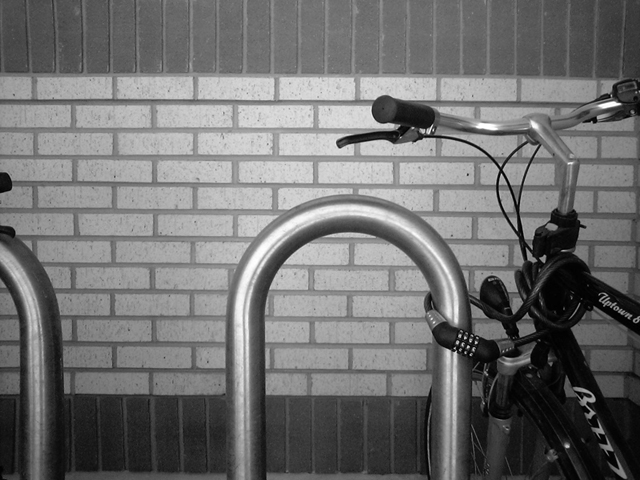
\includegraphics[width=\linewidth]{Bikesgray.jpg}
%  \caption{Original}
%  \label{fig:3}
%\end{subfigure}
%
%\medskip
%\begin{subfigure}{0.4\textwidth}
%  \includegraphics[width=\linewidth]{2/sobel.png}
%  \caption{Sobel}
%  \label{fig:1}
%\end{subfigure}\hfil % <-- added
%\begin{subfigure}{0.4\textwidth}
%  \includegraphics[width=\linewidth]{2/prewitt.png}
%  \caption{Prewitt}
%  \label{fig:3}
%\end{subfigure}
%
%\medskip
%\begin{subfigure}{0.4\textwidth}
%  \includegraphics[width=\linewidth]{2/laplace.png}
%  \caption{Laplace}
%  \label{fig:4}
%\end{subfigure}\hfil % <-- added
%\begin{subfigure}{0.4\textwidth}
%  \includegraphics[width=\linewidth]{2/canny.png}
%  \caption{Canny}
%  \label{fig:6}
%\end{subfigure}
%\caption{Kết quả khi thực hiện các thuật toán với ảnh thứ hai.}
%\label{fig:images}
%\end{figure}
%
%
%\begin{figure}[H]
%    \centering % <-- added
%    \begin{subfigure}{0.4\textwidth}
%  \includegraphics[width=\linewidth]{triangle.png}
%  \caption{Original}
%  \label{fig:3}
%\end{subfigure}
%
%\medskip
%\begin{subfigure}{0.4\textwidth}
%  \includegraphics[width=\linewidth]{3/sobel.png}
%  \caption{Sobel}
%  \label{fig:1}
%\end{subfigure}\hfil % <-- added
%\begin{subfigure}{0.4\textwidth}
%  \includegraphics[width=\linewidth]{3/prewitt.png}
%  \caption{Prewitt}
%  \label{fig:3}
%\end{subfigure}
%
%\medskip
%\begin{subfigure}{0.4\textwidth}
%  \includegraphics[width=\linewidth]{3/laplace.png}
%  \caption{Laplace}
%  \label{fig:4}
%\end{subfigure}\hfil % <-- added
%\begin{subfigure}{0.4\textwidth}
%  \includegraphics[width=\linewidth]{3/canny.png}
%  \caption{Canny}
%  \label{fig:6}
%\end{subfigure}
%\caption{Kết quả khi thực hiện các thuật toán với ảnh thứ ba.}
%\label{fig:images}
%\end{figure}
%
%
%\begin{figure}[H]
%    \centering % <-- added
%    \begin{subfigure}{0.4\textwidth}
%  \includegraphics[width=\linewidth]{traffic.png}
%  \caption{Original}
%  \label{fig:3}
%\end{subfigure}
%
%\medskip
%\begin{subfigure}{0.4\textwidth}
%  \includegraphics[width=\linewidth]{4/sobel.png}
%  \caption{Sobel}
%  \label{fig:1}
%\end{subfigure}\hfil % <-- added
%\begin{subfigure}{0.4\textwidth}
%  \includegraphics[width=\linewidth]{4/prewitt.png}
%  \caption{Prewitt}
%  \label{fig:3}
%\end{subfigure}
%
%\medskip
%\begin{subfigure}{0.4\textwidth}
%  \includegraphics[width=\linewidth]{4/laplace.png}
%  \caption{Laplace}
%  \label{fig:4}
%\end{subfigure}\hfil % <-- added
%\begin{subfigure}{0.4\textwidth}
%  \includegraphics[width=\linewidth]{4/canny.png}
%  \caption{Canny}
%  \label{fig:6}
%\end{subfigure}
%\caption{Kết quả khi thực hiện các thuật toán với ảnh thứ tư.}
%\label{fig:images}
%\end{figure}
%
%
%\begin{figure}[H]
%    \centering % <-- added
%    \begin{subfigure}{0.4\textwidth}
%  \includegraphics[width=\linewidth]{rose.png}
%  \caption{Original}
%  \label{fig:3}
%\end{subfigure}
%
%\medskip
%\begin{subfigure}{0.4\textwidth}
%  \includegraphics[width=\linewidth]{5/sobel.png}
%  \caption{Sobel}
%  \label{fig:1}
%\end{subfigure}\hfil % <-- added
%\begin{subfigure}{0.4\textwidth}
%  \includegraphics[width=\linewidth]{5/prewitt.png}
%  \caption{Prewitt}
%  \label{fig:3}
%\end{subfigure}
%
%\medskip
%\begin{subfigure}{0.4\textwidth}
%  \includegraphics[width=\linewidth]{5/laplace.png}
%  \caption{Laplace}
%  \label{fig:4}
%\end{subfigure}\hfil % <-- added
%\begin{subfigure}{0.4\textwidth}
%  \includegraphics[width=\linewidth]{5/canny.png}
%  \caption{Canny}
%  \label{fig:6}
%\end{subfigure}
%\caption{Kết quả khi thực hiện các thuật toán với ảnh thứ năm.}
%\label{fig:images}
%\end{figure}
%
%\textbf{Nhận xét:}
%\begin{itemize}
%	\item[--] Laplace cho kết quả khá tốt trong trường hợp các đường biên thẳng, trong trường hợp ảnh có nhiễu thị kém hơn các thuật toán còn lại rất nhiều.
%	\item[--] Canny hiển thị đầy đủ hơn các biên có thể có trong ảnh, đồng thời xử lý tốt hơn trong trường hợp ảnh bị nhiễu.
%\end{itemize}
%
%\subsection{Chạy Canny và so sánh với thuật toán được cung cấp bởi OpenCV}
%
%\begin{figure}[H]
%    \centering % <-- added
%\begin{subfigure}{0.4\textwidth}
%  \includegraphics[width=\linewidth]{1/canny.png}
%  \caption{Canny tự viết}
%  \label{fig:1}
%\end{subfigure}\hfil % <-- added
%\begin{subfigure}{0.4\textwidth}
%  \includegraphics[width=\linewidth]{1/cannycv.png}
%  \caption{Canny OpenCV}
%  \label{fig:3}
%\end{subfigure}
%\caption{Ảnh thứ nhất.}
%
%\end{figure}
%
%
%\begin{figure}[H]
%    \centering % <-- added
%\begin{subfigure}{0.4\textwidth}
%  \includegraphics[width=\linewidth]{2/canny.png}
%  \caption{Canny tự viết}
%  \label{fig:1}
%\end{subfigure}\hfil % <-- added
%\begin{subfigure}{0.4\textwidth}
%  \includegraphics[width=\linewidth]{2/cannycv.png}
%  \caption{Canny OpenCV}
%  \label{fig:3}
%\end{subfigure}
%\caption{Ảnh thứ hai.}
%
%\end{figure}
%
%
%\begin{figure}[H]
%    \centering % <-- added
%\begin{subfigure}{0.4\textwidth}
%  \includegraphics[width=\linewidth]{3/canny.png}
%  \caption{Canny tự viết}
%  \label{fig:1}
%\end{subfigure}\hfil % <-- added
%\begin{subfigure}{0.4\textwidth}
%  \includegraphics[width=\linewidth]{3/cannycv.png}
%  \caption{Canny OpenCV}
%  \label{fig:3}
%\end{subfigure}
%\caption{Ảnh thứ ba.}
%
%\end{figure}
%
%
%\begin{figure}[H]
%    \centering % <-- added
%\begin{subfigure}{0.4\textwidth}
%  \includegraphics[width=\linewidth]{4/canny.png}
%  \caption{Canny tự viết}
%  \label{fig:1}
%\end{subfigure}\hfil % <-- added
%\begin{subfigure}{0.4\textwidth}
%  \includegraphics[width=\linewidth]{4/cannycv.png}
%  \caption{Canny OpenCV}
%  \label{fig:3}
%\end{subfigure}
%\caption{Ảnh thứ tư.}
%
%\end{figure}
%
%
%\begin{figure}[H]
%    \centering % <-- added
%\begin{subfigure}{0.4\textwidth}
%  \includegraphics[width=\linewidth]{5/canny.png}
%  \caption{Canny tự viết}
%  \label{fig:1}
%\end{subfigure}\hfil % <-- added
%\begin{subfigure}{0.4\textwidth}
%  \includegraphics[width=\linewidth]{5/cannycv.png}
%  \caption{Canny OpenCV}
%  \label{fig:3}
%\end{subfigure}
%\caption{Ảnh thứ năm.}
%
%\end{figure}
%
%\newpage